\documentclass[11pt,a4paper]{article}

\usepackage[margin=1.1in,headheight=14pt]{geometry}
\usepackage{lmodern}
\usepackage{microtype}
\usepackage{amsmath,amssymb,amsthm}
\usepackage{mathtools}
\usepackage{booktabs}
\usepackage{array}
\usepackage[dvipsnames]{xcolor}
\usepackage{tikz}
\usetikzlibrary{decorations.pathreplacing,arrows.meta,calc}
\usepackage{pgfplots}
\pgfplotsset{compat=1.18}
\usepgfplotslibrary{fillbetween}
\usepackage[font=small,labelfont=bf,margin=0.5cm]{caption}
\usepackage{subcaption}
\usepackage{titlesec}
\usepackage{fancyhdr}
\usepackage[nottoc,notlof,notlot]{tocbibind}
\usepackage[colorlinks=true,linkcolor=MidnightBlue,citecolor=OliveGreen,urlcolor=MidnightBlue]{hyperref}
\hypersetup{
  pdftitle={How long is the graph of x^n? Logarithmic corner defects in arc length},
  pdfauthor={Zishaan Ahmed},
}

% ---------------------------------------------------------------- headings
\titleformat{\section}{\normalfont\Large\bfseries}{\thesection}{0.8em}{}
\titleformat{\subsection}{\normalfont\large\bfseries}{\thesubsection}{0.8em}{}
\titlespacing*{\section}{0pt}{0pt}{1.4em}

% ------------------------------------------------------ float placement
\renewcommand{\topfraction}{0.9}
\renewcommand{\bottomfraction}{0.8}
\renewcommand{\textfraction}{0.07}
\renewcommand{\floatpagefraction}{0.75}
\setcounter{topnumber}{3}
\setcounter{bottomnumber}{2}
\setcounter{totalnumber}{4}
\makeatletter
\setlength{\@fptop}{0pt}
\setlength{\@fpsep}{20pt plus 4pt}
\setlength{\@fpbot}{0pt plus 1fil}
\makeatother

% ------------------------------------------------------- running headers
\pagestyle{fancy}
\fancyhf{}
\fancyhead[L]{\small\itshape How long is the graph of $x^n$?}
\fancyhead[R]{\small\nouppercase{\leftmark}}
\fancyfoot[C]{\small\thepage}
\renewcommand{\headrulewidth}{0.4pt}
\renewcommand{\sectionmark}[1]{\markboth{\thesection\quad #1}{}}

% ------------------------------------------------------------ plot styles
\definecolor{c1}{HTML}{1F4E79}
\definecolor{c2}{HTML}{C0504D}
\definecolor{c3}{HTML}{4F8A3C}
\pgfplotsset{
  paper/.style={
    width=0.94\linewidth, height=0.70\linewidth,
    axis lines=left, tick label style={font=\footnotesize},
    label style={font=\small}, legend style={font=\footnotesize,draw=none,fill=white,fill opacity=0.85,text opacity=1},
    legend cell align=left, every axis plot/.append style={thick},
  },
}

\newtheorem{theorem}{Theorem}[section]
\newtheorem{lemma}[theorem]{Lemma}
\newtheorem{proposition}[theorem]{Proposition}
\newtheorem{corollary}[theorem]{Corollary}
\newtheorem*{mainA}{Theorem A}
\newtheorem*{mainB}{Theorem B}
\newtheorem*{mainC}{Theorem C}
\newtheorem*{mainD}{Theorem D}
\theoremstyle{definition}
\newtheorem{definition}[theorem]{Definition}
\newtheorem{question}{Question}
\theoremstyle{remark}
\newtheorem{remark}[theorem]{Remark}

\numberwithin{equation}{section}

\newcommand{\eps}{\varepsilon}
\newcommand{\dd}{\,\mathrm{d}}
\newcommand{\R}{\mathbb{R}}

\begin{document}

% =================================================================== title
\begin{titlepage}
\centering
\vspace*{2.2cm}
{\LARGE\bfseries How long is the graph of $\boldsymbol{x^n}$?\par}
\vspace{0.5cm}
{\Large Logarithmic corner defects in arc length\par}
\vspace{1.6cm}
{\large Zishaan Ahmed\par}
\vspace{0.2cm}
{\normalsize\href{mailto:iamzishaan@gmail.com}{\texttt{iamzishaan@gmail.com}}\par}
\vspace{0.6cm}
{\normalsize September 2026\par}
\vspace{1.8cm}

\begin{minipage}{0.86\textwidth}
\small
\begin{center}\textbf{Abstract}\end{center}
\vspace{0.2cm}
\noindent
The graph of $y=x^n$ on $[0,1]$ has arc length $L(n)$ that tends to $2$ as
$n\to\infty$, because the curve hugs the two legs of the corner
$(0,0)\to(1,0)\to(1,1)$. We determine exactly how fast. We prove
\begin{gather*}
  2-L(n)=\frac{\ln n+1-\ln 2}{n-1}+O\!\left(\frac{\ln^2 n}{n^2}\right),\\
  L(n)=1+\Bigl(\frac{2}{e\,n}\Bigr)^{1/(n-1)}+\frac{\pi^2}{12\,n^2}
  +O\!\left(\frac{\ln n}{n^3}\right).
\end{gather*}
Both statements follow from an exact, rapidly convergent formula for $L(n)$
involving only the Gamma function, which we obtain from a single Beta
integral. The factor $\ln n$ has a simple geometric cause: $x^n$ spends a
horizontal distance of about $(\ln n)/n$ climbing steeply. The phenomenon persists for corners of
any turning angle $\theta$: the coefficient of $(\ln n)/n$ becomes
$2\sin^2(\theta/2)$, and we compute the next constant in closed form. For
contrast, we show that the perimeter of the ``squircle''
$|x|^p+|y|^p=1$ approaches $8$ \emph{without} a logarithm:
$P(p)=8-4K/p+O(p^{-2})$ with $K=2\sqrt2\,\ln(1+\sqrt2)-2\ln 2$. All
results are elementary and accessible to a reader who knows calculus
and the Gamma function.

\vspace{0.8cm}
\noindent\textbf{Keywords:} arc length, asymptotic expansion, Mellin transform,
Beta integral, superellipse.

\vspace{0.2cm}
\noindent\textbf{MSC 2020:} 26A06, 41A60, 33B15, 53A04.
\end{minipage}

\vfill
{\footnotesize Code and \LaTeX{} source:
\url{https://github.com/zishaan1911/arc-length-of-xn}\par}
\end{titlepage}

% ============================================================ front matter
\pagenumbering{roman}
\pagestyle{plain}
\tableofcontents
\vspace{1.2cm}
\listoffigures
\vspace{1.2cm}
\listoftables
\clearpage
\pagestyle{fancy}
\pagenumbering{arabic}

% every numbered section from here on starts on a new page
\newcommand{\sectionbreak}{\clearpage}

%======================================================================
\section{Introduction}
%======================================================================

A classic warning in calculus concerns the ``staircase paradox'': a
staircase from $(0,0)$ to $(1,1)$ with ever finer steps converges uniformly
to the diagonal, yet its length stays equal to $2$ rather than approaching
$\sqrt2$. Arc length is not continuous under uniform convergence; it is only
lower semicontinuous~\cite{BBI}.

The family $y=x^n$ on $[0,1]$ exhibits a similar effect, in a smooth and more
subtle form. As $n\to\infty$ the graphs converge (in the Hausdorff sense) to
the ``corner'' path
\[
  \Gamma:\ (0,0)\longrightarrow(1,0)\longrightarrow(1,1),
\]
and this time the lengths do converge to the length of the limit:
\[
  L(n):=\int_0^1\sqrt{1+n^2x^{2n-2}}\dd x\ \longrightarrow\ 2 .
\]
This is a common exercise. The question we answer here is:
\emph{how fast?} The answer turns out to be surprisingly rich (see
Figure~\ref{fig:curves}).

\begin{figure}[!htbp]
\centering
\begin{subfigure}{0.47\textwidth}
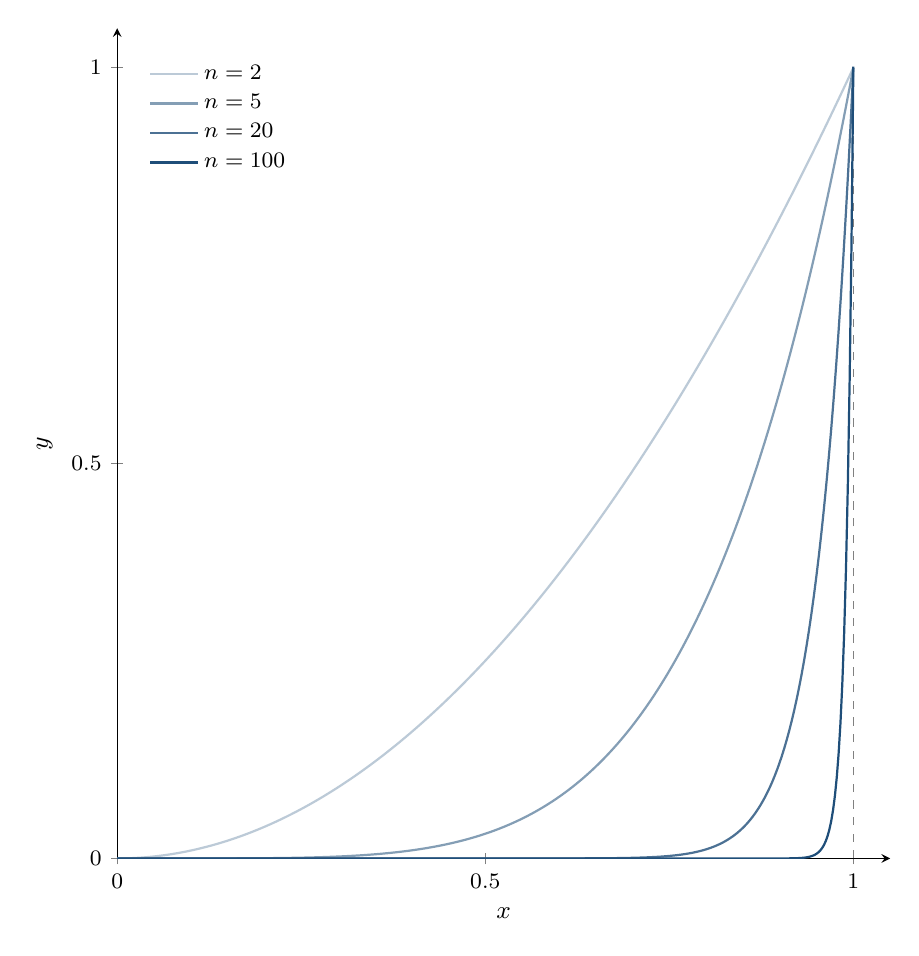
\begin{tikzpicture}
\begin{axis}[paper, height=\linewidth, xmin=0, xmax=1.05, ymin=0, ymax=1.05,
  xlabel={$x$}, ylabel={$y$}, legend pos=north west, xtick={0,0.5,1}, ytick={0,0.5,1}]
  \draw[gray, dashed] (axis cs:1,0) -- (axis cs:1,1);
  \addplot[c1!30, domain=0:1, samples=150] {x^2};
  \addplot[c1!55, domain=0:1, samples=200] {x^5};
  \addplot[c1!80, domain=0:1, samples=300] {x^20};
  \addplot[c1, domain=0:1, samples=400] {x^100};
  \legend{$n=2$, $n=5$, $n=20$, $n=100$}
\end{axis}
\end{tikzpicture}
\subcaption{Graphs of $y=x^n$.}
\end{subfigure}\hfill
\begin{subfigure}{0.47\textwidth}
\begin{tikzpicture}
\begin{axis}[paper, height=\linewidth, xmin=0, xmax=1.05, ymin=0, ymax=1.05,
  xlabel={$x$}, ylabel={$y$}, legend pos=south west, xtick={0,0.5,1}, ytick={0,0.5,1}]
  \draw[gray, dashed] (axis cs:1,0) -- (axis cs:1,1) -- (axis cs:0,1);
  \addplot[c2!30, domain=0:1, samples=150, variable=t] ({t^(1/2)}, {(1-t)^(1/2)});
  \addplot[c2!55, domain=0:1, samples=200, variable=t] ({t^(1/4)}, {(1-t)^(1/4)});
  \addplot[c2!80, domain=0:1, samples=300, variable=t] ({t^(1/10)}, {(1-t)^(1/10)});
  \addplot[c2, domain=0:1, samples=400, variable=t] ({t^(1/40)}, {(1-t)^(1/40)});
  \legend{$p=2$, $p=4$, $p=10$, $p=40$}
\end{axis}
\end{tikzpicture}
\subcaption{Quarter squircles $x^p+y^p=1$.}
\end{subfigure}
\caption[Two families of curves collapsing onto a right-angled corner]{Two families
of curves that collapse onto a right-angled corner (dashed). In (a) the length defect is of
order $(\ln n)/n$ (Theorems~A and~B). In (b) it is of order $1/p$ (Theorem~D).}
\label{fig:curves}
\end{figure}

\subsection{Main results}
Throughout, $n>1$ is real, $\ln$ is the natural logarithm, and we write
\[
  \eps:=\frac1{n-1}, \qquad D(n):=2-L(n).
\]
Our first result is an elementary estimate, with explicit constants.

\begin{mainA}[Proposition~\ref{prop:elementary}]
For every $n\ge 3$,
\[
  \frac{\ln n-1}{n-1}-\frac{\ln^2 n}{2(n-1)^2}\ \le\ 2-L(n)\ \le\ \frac{\ln n+1}{n-1}.
\]
In particular $2-L(n)\sim (\ln n)/n$.
\end{mainA}

The second result is exact. Let
\begin{equation}\label{eq:Rdef}
  R(\eps):=\frac{\Gamma\!\left(1+\frac{\eps}{2}\right)\Gamma\!\left(\frac{1-\eps}{2}\right)}{\sqrt\pi\,(1+\eps)},
  \qquad 0\le \eps<1,
\end{equation}
so that $R(0)=1$.

\begin{mainB}[Theorem~\ref{thm:exact}, Corollary~\ref{cor:asymp}]
For every real $n>2$, with $\eps=1/(n-1)$,
\begin{equation}\label{eq:exact-intro}
  L(n)=1+\frac{R(\eps)}{n^{\eps}}
  -\sum_{k=1}^{\infty}\binom{1/2}{k}\frac{1}{n^{2k-1}\bigl((2k-1)(n-1)-1\bigr)} .
\end{equation}
Consequently
\begin{align}
  L(n)&=2-\frac{\ln n+1-\ln2}{n-1}+O\!\left(\frac{\ln^2n}{n^2}\right), \label{eq:asy1}\\
  L(n)&=1+\Bigl(\frac{2}{e\,n}\Bigr)^{1/(n-1)}+\frac{\pi^2}{12\,n^2}+O\!\left(\frac{\ln n}{n^3}\right). \label{eq:asy2}
\end{align}
\end{mainB}

The terms of the series in~\eqref{eq:exact-intro} decay like $n^{-2k}$. Four
terms already give $L(100)$ to about 22 digits. Formula~\eqref{eq:asy2} is
remarkably accurate: at $n=100$ its error is below $5\times10^{-6}$
(Table~\ref{tab:xn}).

Where does $\ln n$ come from? Section~\ref{sec:why} explains that it is a
feature of how $x^n$ approaches the \emph{vertical} leg of the corner.
Section~\ref{sec:angle} shows that it does not depend on the corner being a
right angle. For unit vectors
$u,v$ making an angle $\theta\in[0,\pi)$, consider the curve
$\gamma_n(x)=x\,u+x^n\,v$, $0\le x\le1$, which collapses onto the
two-segment path with legs $u$ and $v$ (total length $2$) as $n\to\infty$.
The graph of $x^n$ is the case $\theta=\pi/2$.

\begin{mainC}[Theorem~\ref{thm:angle}]
Let $L_\theta(n)$ be the length of $\gamma_n$. Then
\[
  2-L_\theta(n)=\frac{2\sin^2(\theta/2)\,\ln n+C(\theta)}{n-1}+O\!\left(\frac{\ln^2 n}{n^2}\right),
  \qquad
  C(\theta)=2\sin^2\tfrac{\theta}{2}+4\cos^2\tfrac{\theta}{2}\,\ln\cos\tfrac{\theta}{2}.
\]
\end{mainC}

Finally, the logarithm is \emph{not} a universal feature of curves
collapsing onto a corner. The superellipse (or ``squircle'')
$|x|^p+|y|^p=1$, popularized by Piet Hein~\cite{Gardner}, converges to the
square $[-1,1]^2$ as $p\to\infty$, but more quickly.

\begin{mainD}[Theorem~\ref{thm:squircle}]
The perimeter $P(p)$ of $|x|^p+|y|^p=1$ satisfies, for $p\ge 2$,
\[
  \Bigl|\,P(p)-\Bigl(8-\frac{4K}{p}\Bigr)\Bigr|\le\frac{12}{p^2},
  \qquad K=2\sqrt2\,\ln\bigl(1+\sqrt2\bigr)-2\ln2=1.10660\ldots .
\]
\end{mainD}

Table~\ref{tab:summary} collects these results.

\begin{table}[!htbp]
\centering
\caption[Summary of the main results]{Summary of the main results. In each case the curve
collapses onto a two-segment path, and the \emph{defect} is the limiting length minus the
actual length.}\label{tab:summary}
\renewcommand{\arraystretch}{1.6}
\begin{tabular}{>{\raggedright}p{3.9cm}ccl}
\toprule
Curve & Limit & Defect & Where\\
\midrule
$y=x^n$, $0\le x\le1$ & $2$ & $\dfrac{\ln n+1-\ln2}{n-1}+O\Bigl(\dfrac{\ln^2n}{n^2}\Bigr)$ &
  Thm.~\ref{thm:exact}, Cor.~\ref{cor:asymp}\\
$x\,u+x^n\,v$, angle $\theta$ between $u,v$ & $2$ &
  $\dfrac{2\sin^2\frac\theta2\,\ln n+C(\theta)}{n-1}+O\Bigl(\dfrac{\ln^2n}{n^2}\Bigr)$ &
  Thm.~\ref{thm:angle}\\
squircle $|x|^p+|y|^p=1$ (perimeter) & $8$ & $\dfrac{4K}{p}+O\Bigl(\dfrac{1}{p^2}\Bigr)$ &
  Thm.~\ref{thm:squircle}\\
\bottomrule
\end{tabular}
\end{table}

\subsection{Related work and what is new}
The limit $L(n)\to2$ is standard. The indefinite arc-length integral of
$x^n$ is known to be a Gauss hypergeometric function; see the discussion
in~\cite{MSE}, which gives in particular
\begin{equation}\label{eq:hyp}
  L(n)={}_2F_1\!\left(-\tfrac12,\tfrac{\eps}{2};\,1+\tfrac{\eps}{2};\,-n^2\right).
\end{equation}
In principle, \eqref{eq:exact-intro} can be obtained from~\eqref{eq:hyp}
through the classical connection formula that transforms a ${}_2F_1$ at
argument $z$ into functions of $1/z$~\cite[15.8.2]{DLMF} (see
Remark~\ref{rem:hyp}). Our derivation avoids hypergeometric functions
entirely. It uses one substitution and one Beta integral, and it leads
directly to the asymptotic
statements~\eqref{eq:asy1}--\eqref{eq:asy2}, which we have not found in
the literature. Two recent preprints~\cite{MRL,RM} give hypergeometric
series representations for the arc length of supercircles and the
perimeter of Lam\'e superellipses, and they verify the limiting value $8$
as $p\to\infty$. They do not give the rate $4K/p$ of Theorem~D, and we did
not find it elsewhere either. Given how elementary these questions are, some
of our results may well exist as solved problems in the journal literature.
We would welcome references.

\subsection{Organization}
Section~\ref{sec:defect} reduces every result to a single one-dimensional
integral. Section~\ref{sec:elementary} proves Theorem~A,
Section~\ref{sec:exact} proves the exact formula, and
Section~\ref{sec:asymp} extracts the asymptotics. Section~\ref{sec:angle}
treats general angles, Section~\ref{sec:squircle} treats the squircle, and
Section~\ref{sec:why} explains the difference between the two
behaviors. Section~\ref{sec:conclusion} summarizes and lists open questions.

%======================================================================
\section{The taxicab defect}\label{sec:defect}
%======================================================================

The key idea is to compare Euclidean length with \emph{taxicab} length. Let
$\gamma(t)=(x(t),y(t))$ be a $C^1$ curve whose two coordinates are each
monotone, joining $(0,0)$ to $(1,1)$. Its taxicab length is
$\int(|x'|+|y'|)\dd t=1+1=2$. Hence
\begin{equation}\label{eq:taxicab}
  2-\operatorname{length}(\gamma)=\int\Bigl(|x'|+|y'|-\sqrt{x'^2+y'^2}\Bigr)\dd t\ \ge 0 .
\end{equation}
The integrand is nonnegative. It vanishes where the curve is horizontal or
vertical and is largest where the curve moves diagonally. Thus $2-L(n)$
measures how much ``diagonal travel'' the curve does. The same idea works
for any pair of directions.

\begin{lemma}[Defect integral]\label{lem:defect}
Let $u,v\in\R^2$ be unit vectors with $u\cdot v=c=\cos\theta$, where
$\theta\in[0,\pi)$. Let $n>1$, $\eps=1/(n-1)$, and
$\gamma_n(x)=x\,u+x^n\,v$ for $0\le x\le 1$. Then
\begin{equation}\label{eq:defect}
  2-\operatorname{length}(\gamma_n)=\eps\,n^{-\eps}\int_0^n h_c(s)\,s^{\eps-1}\dd s,
\end{equation}
where
\begin{equation}\label{eq:hc}
  h_c(s):=1+s-\sqrt{1+2cs+s^2}=\frac{2(1-c)\,s}{1+s+\sqrt{1+2cs+s^2}}\ \ \ (s\ge0).
\end{equation}
\end{lemma}

\begin{proof}
Write $y=x^n$. Then $\gamma_n'=u+y'v$ and $|\gamma_n'|=\sqrt{1+2cy'+y'^2}$.
Since $\int_0^1 y'\dd x=1$,
\[
  2-\operatorname{length}(\gamma_n)=\int_0^1\bigl(1+y'-|u+y'v|\bigr)\dd x=\int_0^1 h_c\bigl(nx^{n-1}\bigr)\dd x.
\]
Now substitute $s=nx^{n-1}$. This is an increasing bijection $(0,1]\to(0,n]$,
with $x=(s/n)^{\eps}$ and $\dd x=\eps\,(s/n)^{\eps}\,\dd s/s$. This
gives~\eqref{eq:defect}. The second expression in~\eqref{eq:hc} comes from
multiplying and dividing by $1+s+\sqrt{1+2cs+s^2}$.
\end{proof}

The graph of $x^n$ is the case $u=(1,0)$, $v=(0,1)$, $c=0$. We write
\begin{equation}\label{eq:D}
  g(s):=h_0(s)=1+s-\sqrt{1+s^2},
  \qquad
  D(n)=2-L(n)=\eps\,n^{-\eps}\int_0^n g(s)\,s^{\eps-1}\dd s.
\end{equation}
Two features of $g$ drive everything that follows. First, $g(s)\approx s$ for small $s$, so
gentle slopes cost little. Second, $g(s)\to1$ as $s\to\infty$, so steep slopes cost the full
horizontal distance. It is this second feature that makes $\int^n g(s)\,\dd s/s$
grow like $\ln n$. Figure~\ref{fig:g} in Section~\ref{sec:elementary} shows $g$
together with two elementary bounds.

%======================================================================
\section{Elementary bounds}\label{sec:elementary}
%======================================================================

\begin{proposition}\label{prop:elementary}
For every real $n\ge3$,
\[
  \frac{\ln n-1}{n-1}-\frac{\ln^2 n}{2(n-1)^2}\ \le\ D(n)\ \le\ \frac{\ln n+1}{n-1}.
\]
\end{proposition}

\begin{proof}
We need two bounds on $g$. Since $1+s+\sqrt{1+s^2}\ge 1+s+\max(1,s)\ge2\max(1,s)$,
the formula $g(s)=2s/(1+s+\sqrt{1+s^2})$ gives
\begin{equation}\label{eq:gupper}
  0\le g(s)\le\min(s,1).
\end{equation}
Also $g(s)=1-\bigl(\sqrt{1+s^2}-s\bigr)=1-\dfrac{1}{s+\sqrt{1+s^2}}$. Hence
\begin{equation}\label{eq:glower}
  g(s)\ge 1-\frac1{2s}\qquad(s>0).
\end{equation}

\emph{Upper bound.} By~\eqref{eq:gupper},
\[
  \int_0^n g(s)s^{\eps-1}\dd s\le\int_0^1 s^{\eps}\dd s+\int_1^n s^{\eps-1}\dd s=\frac1{1+\eps}+\frac{n^{\eps}-1}{\eps}.
\]
Multiplying by $\eps n^{-\eps}$ gives
$D(n)\le\eps+(1-n^{-\eps})\le\eps+\eps\ln n$, because
$1-e^{-x}\le x$.

\emph{Lower bound.} We drop the (nonnegative) integral over $[0,1]$ and
use~\eqref{eq:glower} on $[1,n]$:
\[
  D(n)\ge\eps n^{-\eps}\int_1^n\Bigl(s^{\eps-1}-\tfrac12 s^{\eps-2}\Bigr)\dd s
  =(1-n^{-\eps})-\frac{\eps\, n^{-\eps}}{2}\cdot\frac{1-n^{\eps-1}}{1-\eps}
  \ge(1-n^{-\eps})-\frac{\eps}{2(1-\eps)}.
\]
For $n\ge3$ we have $\eps\le\frac12$, so $\eps/(2(1-\eps))\le\eps$. Finally,
$1-e^{-x}\ge x-x^2/2$ for $x\ge0$. With $x=\eps\ln n$, this gives the claim.
\end{proof}

\begin{figure}[!htbp]
\centering
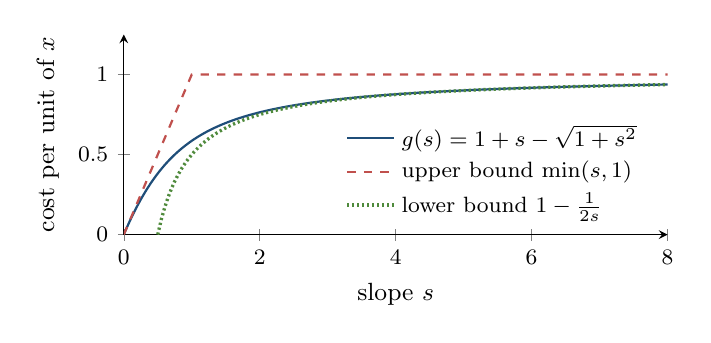
\begin{tikzpicture}
\begin{axis}[paper, width=0.7\textwidth, height=0.34\textwidth, xmin=0, xmax=8, ymin=0, ymax=1.25,
  xlabel={slope $s$}, ylabel={cost per unit of $x$}, legend pos=south east]
  \addplot[c1, domain=0:8, samples=200] {1+x-sqrt(1+x^2)};
  \addplot[c2, dashed, domain=0:8, samples=161] {min(x,1)};
  \addplot[c3, densely dotted, very thick, domain=0.5:8, samples=150] {1-1/(2*x)};
  \legend{{$g(s)=1+s-\sqrt{1+s^2}$}, {upper bound $\min(s,1)$}, {lower bound $1-\frac{1}{2s}$}}
\end{axis}
\end{tikzpicture}
\caption[The defect density $g(s)$ and its elementary bounds]{The defect density $g(s)$: the
length lost per unit of horizontal distance along a stretch of slope $s$. Gentle slopes lose
almost nothing; steep slopes lose almost the whole horizontal step. The bounds are
\eqref{eq:gupper} and \eqref{eq:glower}.}
\label{fig:g}
\end{figure}

Proposition~\ref{prop:elementary} already shows that $n\,(2-L(n))/\ln n\to1$.
The bounds leave room for the \emph{constant} next to $\ln n$ anywhere in
$[-1,1]$. Section~\ref{sec:asymp} shows that this constant is $1-\ln2\approx0.307$.

%======================================================================
\section{An exact formula}\label{sec:exact}
%======================================================================

The function $k(s):=\sqrt{1+s^2}-s=1-g(s)$ is positive and decreasing, with $k(0)=1$ and
$k(s)\le 1/(2s)$. Therefore its \emph{Mellin transform}
\[
  M(\eps):=\int_0^\infty k(s)\,s^{\eps-1}\dd s
\]
converges for $0<\eps<1$. Mellin transforms are the natural tool for
integrals like~\eqref{eq:D}; see~\cite{FGD} for a survey. Here, however, we
need only one explicit evaluation.

\begin{lemma}\label{lem:mellin}
For $0<\eps<1$,
\[
  \eps\,M(\eps)=R(\eps)=\frac{\Gamma\!\left(1+\frac{\eps}{2}\right)\Gamma\!\left(\frac{1-\eps}{2}\right)}{\sqrt\pi\,(1+\eps)}.
\]
\end{lemma}

\begin{proof}
Put $w=k(s)=\sqrt{1+s^2}-s$. As $s$ runs over $(0,\infty)$, $w$ decreases
from $1$ to $0$. Solving gives $s=(1-w^2)/(2w)$ and $\dd s=-\frac{1+w^2}{2w^2}\dd w$. Thus
\[
  M(\eps)=\int_0^1 w\Bigl(\frac{1-w^2}{2w}\Bigr)^{\eps-1}\frac{1+w^2}{2w^2}\dd w
  =2^{-\eps}\int_0^1(1-w^2)^{\eps-1}\,w^{-\eps}\,(1+w^2)\dd w.
\]
Substituting $w=\sqrt{t}$ gives the Euler Beta integral
$B(a,b)=\int_0^1t^{a-1}(1-t)^{b-1}\dd t$ \cite[5.12.1]{DLMF}:
\[
  M(\eps)=2^{-\eps-1}\int_0^1(1-t)^{\eps-1}\bigl(t^{-\frac{1+\eps}{2}}+t^{\frac{1-\eps}{2}}\bigr)\dd t
  =2^{-\eps-1}\Bigl[B\bigl(\tfrac{1-\eps}{2},\eps\bigr)+B\bigl(\tfrac{3-\eps}{2},\eps\bigr)\Bigr].
\]
Write $B(a,b)=\Gamma(a)\Gamma(b)/\Gamma(a+b)$ and use $\Gamma(z+1)=z\Gamma(z)$,
which gives $\Gamma(\frac{3\pm\eps}2)=\frac{1\pm\eps}{2}\Gamma(\frac{1\pm\eps}{2})$. The
bracket then becomes
\[
  \frac{\Gamma(\eps)\Gamma(\frac{1-\eps}{2})}{\Gamma(\frac{1+\eps}{2})}\Bigl(1+\frac{1-\eps}{1+\eps}\Bigr)
  =\frac{\Gamma(\eps)\Gamma(\frac{1-\eps}{2})}{\Gamma(\frac{3+\eps}{2})}.
\]
Hence
$\eps M(\eps)=\Gamma(1+\eps)\Gamma(\frac{1-\eps}2)\big/\bigl(2^{1+\eps}\Gamma(\frac{3+\eps}2)\bigr)$.
Legendre's duplication formula
$\Gamma(1+\eps)=\pi^{-1/2}2^{\eps}\,\Gamma(\frac{1+\eps}{2})\Gamma(1+\frac{\eps}{2})$
\cite[5.5.5]{DLMF}, together with
$\Gamma(\frac{3+\eps}{2})=\frac{1+\eps}{2}\Gamma(\frac{1+\eps}{2})$, turns this into the stated form.
\end{proof}

\begin{theorem}\label{thm:exact}
For every real $n>2$, with $\eps=1/(n-1)$,
\[
  L(n)=1+\frac{R(\eps)}{n^{\eps}}
  -\sum_{k=1}^{\infty}\binom{1/2}{k}\frac{1}{n^{2k-1}\bigl((2k-1)(n-1)-1\bigr)},
\]
where $\binom{1/2}{k}=\frac{(1/2)(-1/2)\cdots(3/2-k)}{k!}$, so the coefficients are
$\frac12,-\frac18,\frac1{16},-\frac5{128},\dots$ The series converges
absolutely.
\end{theorem}

\begin{proof}
Since $n>2$, we have $0<\eps<1$. By~\eqref{eq:D} and $g=1-k$,
\[
  \int_0^n g(s)s^{\eps-1}\dd s=\frac{n^{\eps}}{\eps}-\int_0^\infty k(s)s^{\eps-1}\dd s+\int_n^\infty k(s)s^{\eps-1}\dd s .
\]
Multiplying by $\eps n^{-\eps}$ and applying Lemma~\ref{lem:mellin} gives
\[
  D(n)=1-\frac{R(\eps)}{n^{\eps}}+\eps\,n^{-\eps}\int_n^\infty k(s)\,s^{\eps-1}\dd s .
\]
For $s>1$, the binomial series gives
$k(s)=s\bigl(\sqrt{1+s^{-2}}-1\bigr)=\sum_{k\ge1}\binom{1/2}{k}s^{1-2k}$. Because
$\sum_k|\binom{1/2}{k}|\,n^{-2k}<\infty$ for $n>1$, we may integrate term by
term on $[n,\infty)$ (by the Weierstrass $M$-test, or Tonelli's theorem). Each term gives
$\int_n^\infty s^{\eps-2k}\dd s=n^{\eps+1-2k}/(2k-1-\eps)$. Hence
\[
  \eps\, n^{-\eps}\int_n^\infty k(s)s^{\eps-1}\dd s=\sum_{k\ge1}\binom{1/2}{k}\frac{\eps\,n^{1-2k}}{2k-1-\eps}
  =\sum_{k\ge1}\binom{1/2}{k}\frac{1}{n^{2k-1}\bigl((2k-1)(n-1)-1\bigr)} .
\]
Finally, $L(n)=2-D(n)$.
\end{proof}

\begin{remark}[The case $n=2$]
At $n=2$ we have $\eps=1$. Both $R(\eps)$ (through $\Gamma(\frac{1-\eps}{2})$) and the
$k=1$ term of the series have poles, and the two poles cancel. The limit
$n\to2^+$ of the formula recovers the length of the parabola,
$L(2)=\frac{\sqrt5}{2}+\frac14\ln(2+\sqrt5)$.
\end{remark}

\begin{remark}[Scaled curves]\label{rem:scaled}
The same proof applies without change to $y=c\,x^n$ on $[0,1]$ for any $c>0$ with
$cn>1$. The only difference is that the substitution now ends at $s=cn$:
\[
  \operatorname{length}\bigl(c\,x^n\bigr)=c+\frac{R(\eps)}{(cn)^{\eps}}
  -\sum_{k\ge1}\binom{1/2}{k}\frac{1}{(cn)^{2k-1}\bigl((2k-1)(n-1)-1\bigr)}.
\]
Scaling shows that the length of $y=x^n$ on $[0,a]$ equals $a$ times the
length of $a^{n-1}x^n$ on $[0,1]$, so this also covers all intervals $[0,a]$.
\end{remark}

\begin{remark}[Relation to the hypergeometric form]\label{rem:hyp}
The large-argument
connection formula~\cite[15.8.2]{DLMF} expresses~\eqref{eq:hyp} as a
combination of two ${}_2F_1$'s at argument $-1/n^2$. One can check that the Gamma
factor multiplying $n^{-\eps}$ there,
$\Gamma(1+\frac\eps2)\Gamma(-\frac{1+\eps}{2})/\Gamma(-\frac12)$, equals
$R(\eps)$. What the present approach adds is an elementary route, and
above all the asymptotic consequences in the next section.
\end{remark}

%======================================================================
\section{Asymptotic expansion}\label{sec:asymp}
%======================================================================

We need the Taylor expansion of $\ln R$ at $0$. It uses the classical values
$\psi(1)=-\gamma$, $\psi(\tfrac12)=-\gamma-2\ln2$, $\psi'(1)=\pi^2/6$,
$\psi'(\tfrac12)=\pi^2/2$, $\psi''(1)=-2\zeta(3)$, and
$\psi''(\tfrac12)=-14\zeta(3)$ \cite[\S5.4, \S5.15]{DLMF}, where
$\psi=\Gamma'/\Gamma$.

\begin{lemma}\label{lem:logR}
As $\eps\to0$,
\[
  \ln R(\eps)=(\ln2-1)\,\eps+\Bigl(\frac{\pi^2}{12}+\frac12\Bigr)\eps^2+\Bigl(\frac{\zeta(3)}4-\frac13\Bigr)\eps^3+O(\eps^4).
\]
\end{lemma}

\begin{proof}
We have
$\ln R(\eps)=\ln\Gamma(1+\frac\eps2)+\ln\Gamma(\frac{1-\eps}{2})-\frac12\ln\pi-\ln(1+\eps)$, and $R$ is
analytic near $0$. The $j$-th Taylor coefficient of $\ln\Gamma(a+b\eps)$ is
$b^j\psi^{(j-1)}(a)/j!$.
\begin{itemize}
\item \emph{Linear term:} $\frac12\psi(1)-\frac12\psi(\frac12)-1=\ln 2-1$.
\item \emph{Quadratic term:} $\frac18\psi'(1)+\frac18\psi'(\frac12)+\frac12=\frac{\pi^2}{48}+\frac{\pi^2}{16}+\frac12$.
\item \emph{Cubic term:} $\frac1{48}\psi''(1)-\frac1{48}\psi''(\frac12)-\frac13=\frac{12\zeta(3)}{48}-\frac13$.
\end{itemize}
The $\gamma$'s cancel in the linear term.
\end{proof}

\begin{corollary}\label{cor:asymp}
As $n\to\infty$,
\begin{align*}
  \text{(a)}\quad & L(n)=2-\frac{\ln n+1-\ln2}{n-1}+O\!\left(\frac{\ln^2n}{n^2}\right),\\
  \text{(b)}\quad & L(n)=1+\Bigl(\frac{2}{e\,n}\Bigr)^{1/(n-1)}+\frac{\pi^2}{12\,n^2}+O\!\left(\frac{\ln n}{n^3}\right).
\end{align*}
\end{corollary}

\begin{proof}
Put $\lambda=\ln n+1-\ln 2$ and $b=\frac{\pi^2}{12}+\frac12$. By Lemma~\ref{lem:logR},
\[
  \frac{R(\eps)}{n^{\eps}}=\exp\bigl(-\eps\lambda+b\eps^2+O(\eps^3)\bigr)
  =e^{-\eps\lambda}\bigl(1+b\eps^2+O(\eps^3)\bigr).
\]
The series in Theorem~\ref{thm:exact} equals $\frac1{2n(n-2)}+O(n^{-4})$.

For (a), note that $e^{-\eps\lambda}=1-\eps\lambda+O(\eps^2\ln^2n)$, and every other
term is $O(n^{-2})$.

For (b), note that $e^{-\eps\lambda}=1+O(\eps\ln n)$, so
$e^{-\eps\lambda}\,b\eps^2=b\eps^2+O(\ln n/n^3)$. Hence
\[
  L(n)=1+e^{-\eps\lambda}+b\eps^2-\frac1{2n(n-2)}+O\!\left(\frac{\ln n}{n^3}\right).
\]
Now $b\eps^2=b/n^2+O(n^{-3})$ and $\frac{1}{2n(n-2)}=\frac1{2n^2}+O(n^{-3})$, and
$b-\frac12=\frac{\pi^2}{12}$. Finally,
$e^{-\eps\lambda}=\exp\bigl(-\frac{\ln n+1-\ln2}{n-1}\bigr)=\bigl(\frac{2}{en}\bigr)^{1/(n-1)}$.
\end{proof}

\begin{remark}
Carrying the expansion one step further in the same way gives
\[
  L(n)=1+\Bigl(\frac{2}{e\,n}\Bigr)^{\frac1{n-1}}+\frac{\pi^2}{12n^2}
  +\frac{d-b\ln n}{n^3}+O\!\left(\frac{\ln^2 n}{n^4}\right),
\]
with $b=\frac{\pi^2}{12}+\frac12$ and
$d=b(1+\ln2)+\frac{\zeta(3)}4-\frac43\approx1.20631$. We have confirmed this
numerically up to $n=10^5$. All further terms can be computed the same way. They
are polynomials in $\ln n$ divided by powers of $n$.
\end{remark}

Figure~\ref{fig:asymp} and Table~\ref{tab:xn} show the approximations at work.
Figure~\ref{fig:asymp}(a) plots the rescaled defect $(n-1)\bigl(2-L(n)\bigr)$ against
$\ln n$. The points lie on the line $\ln n+1-\ln2$ of Corollary~\ref{cor:asymp}(a),
between the elementary bounds of Proposition~\ref{prop:elementary}.
Figure~\ref{fig:asymp}(b) compares the errors of the two approximations in
Corollary~\ref{cor:asymp}.

\begin{figure}[!htbp]
\centering
\begin{subfigure}{0.48\textwidth}
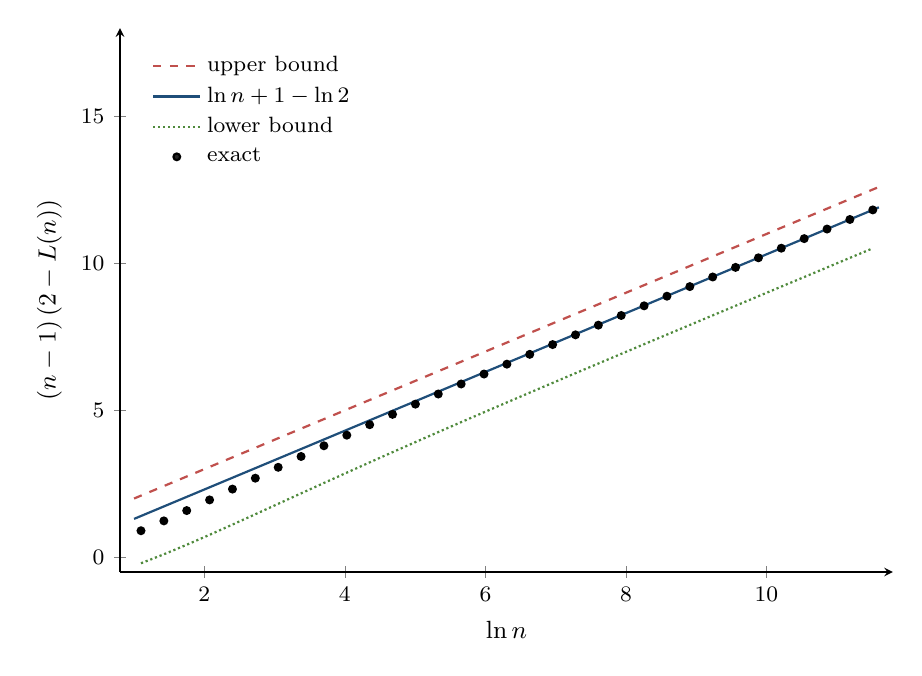
\begin{tikzpicture}
\begin{axis}[paper, xmin=0.8, xmax=11.8, ymin=-0.5, ymax=18,
  xlabel={$\ln n$}, ylabel={$(n-1)\,(2-L(n))$}, legend pos=north west, ytick={0,5,10,15}]
  \addplot[c2, dashed, domain=1:11.6, samples=2] {x+1};
  \addplot[c1, domain=1:11.6, samples=2] {x+1-ln(2)};
  \addplot[c3, densely dotted] coordinates {(1.0986,-0.20312) (1.4241,0.10257) (1.7495,0.42744) (2.075,0.76584) (2.4004,1.1131) (2.7258,1.4655) (3.0513,1.8202) (3.3767,2.1751) (3.7022,2.5289) (4.0276,2.8805) (4.3531,3.2296) (4.6785,3.5759) (5.004,3.9194) (5.3294,4.2603) (5.6549,4.5987) (5.9803,4.935) (6.3058,5.2694) (6.6312,5.6022) (6.9567,5.9336) (7.2821,6.2639) (7.6076,6.5932) (7.933,6.9217) (8.2585,7.2496) (8.5839,7.577) (8.9093,7.904) (9.2348,8.2306) (9.5602,8.557) (9.8857,8.8832) (10.211,9.2092) (10.537,9.5351) (10.862,9.8609) (11.187,10.187) (11.513,10.512)};
  \addplot[only marks, mark=*, mark size=1.2pt, black] coordinates {(1.0986,0.90427) (1.4241,1.2392) (1.7495,1.5907) (2.075,1.9531) (2.4004,2.3214) (2.7258,2.6921) (3.0513,3.0624) (3.3767,3.4304) (3.7022,3.7949) (4.0276,4.1554) (4.3531,4.5115) (4.6785,4.8635) (5.004,5.2114) (5.3294,5.5558) (5.6549,5.8969) (5.9803,6.2353) (6.3058,6.5713) (6.6312,6.9053) (6.9567,7.2377) (7.2821,7.5686) (7.6076,7.8985) (7.933,8.2274) (8.2585,8.5556) (8.5839,8.8832) (8.9093,9.2104) (9.2348,9.5371) (9.5602,9.8636) (9.8857,10.19) (10.211,10.516) (10.537,10.842) (10.862,11.168) (11.187,11.493) (11.513,11.819)};
  \legend{upper bound, $\ln n+1-\ln 2$, lower bound, exact}
\end{axis}
\end{tikzpicture}
\subcaption{Rescaled defect.}
\end{subfigure}\hfill
\begin{subfigure}{0.48\textwidth}
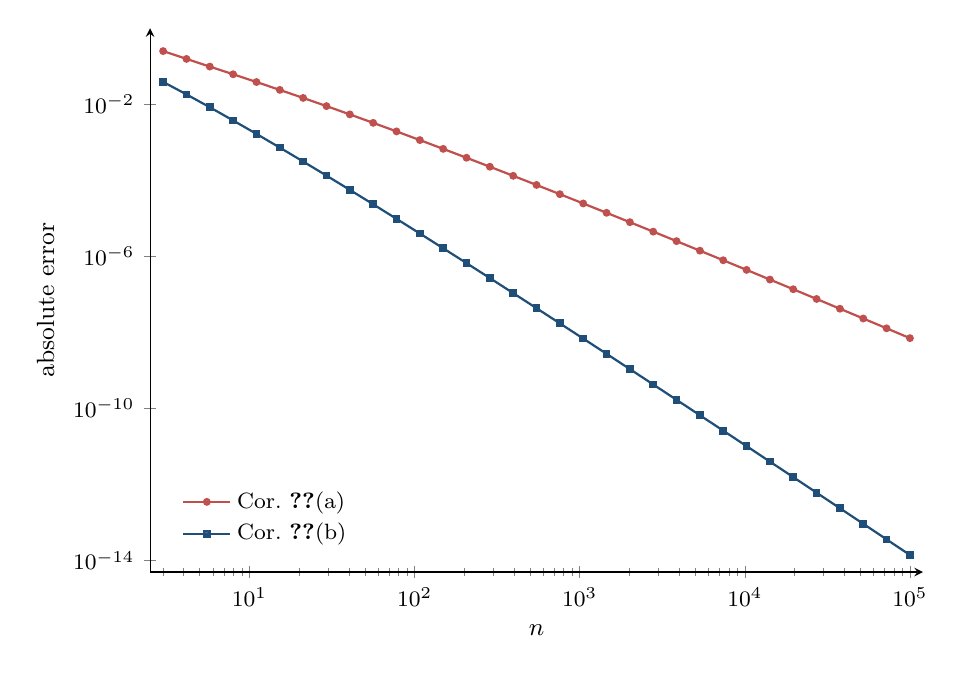
\begin{tikzpicture}
\begin{loglogaxis}[paper, xmin=2.5, xmax=1.2e5, ymin=5e-15, ymax=1,
  xlabel={$n$}, ylabel={absolute error}, legend pos=south west,
  ytick={1e-14,1e-10,1e-6,1e-2}]
  \addplot[c2, mark=*, mark size=1pt] coordinates {(3.0,0.2506) (4.1539,0.1559) (5.7518,0.098) (7.9642,0.06156) (11.028,0.03848) (15.269,0.02387) (21.143,0.01468) (29.275,0.008956) (40.536,0.005416) (56.128,0.003249) (77.718,0.001934) (107.61,0.001144) (149.0,0.0006716) (206.32,0.000392) (285.68,0.0002276) (395.57,0.0001314) (547.72,7.555e-5) (758.4,4.324e-5) (1050.1,2.465e-5) (1454.1,1.4e-5) (2013.4,7.926e-6) (2787.8,4.472e-6) (3860.1,2.516e-6) (5344.9,1.412e-6) (7400.8,7.903e-7) (10248.0,4.413e-7) (14189.0,2.458e-7) (19647.0,1.367e-7) (27204.0,7.585e-8) (37669.0,4.201e-8) (52158.0,2.323e-8) (72220.0,1.282e-8) (1.0e5,7.067e-9)};
  \addplot[c1, mark=square*, mark size=1pt] coordinates {(3.0,0.03875) (4.1539,0.01819) (5.7518,0.008341) (7.9642,0.003753) (11.028,0.001661) (15.269,0.0007249) (21.143,0.0003124) (29.275,0.0001331) (40.536,5.61e-5) (56.128,2.344e-5) (77.718,9.713e-6) (107.61,3.996e-6) (149.0,1.634e-6) (206.32,6.64e-7) (285.68,2.685e-7) (395.57,1.081e-7) (547.72,4.334e-8) (758.4,1.731e-8) (1050.1,6.895e-9) (1454.1,2.738e-9) (2013.4,1.084e-9) (2787.8,4.283e-10) (3860.1,1.688e-10) (5344.9,6.642e-11) (7400.8,2.608e-11) (10248.0,1.023e-11) (14189.0,4.003e-12) (19647.0,1.565e-12) (27204.0,6.107e-13) (37669.0,2.381e-13) (52158.0,9.273e-14) (72220.0,3.607e-14) (1.0e5,1.402e-14)};
  \legend{Cor.~\ref{cor:asymp}(a), Cor.~\ref{cor:asymp}(b)}
\end{loglogaxis}
\end{tikzpicture}
\subcaption{Errors of the two approximations.}
\end{subfigure}
\caption[Accuracy of the asymptotic formulas for $L(n)$]{Accuracy of Corollary~\ref{cor:asymp}.
(a)~The rescaled defect (dots, from Theorem~\ref{thm:exact}) follows the line
$\ln n+1-\ln2$ and stays between the bounds of Proposition~\ref{prop:elementary}.
(b)~The error of (a) decays like $\ln^2 n/n^2$; the error of (b) decays like $\ln n/n^3$.}
\label{fig:asymp}
\end{figure}

\begin{table}[!htbp]
\centering
\caption[Numerical values of $L(n)$ and of its approximations]{The length $L(n)$ of $y=x^n$ on $[0,1]$, computed from
Theorem~\ref{thm:exact} and checked against direct numerical integration for
$n\le1000$, together with the errors of the two approximations in
Corollary~\ref{cor:asymp}.}\label{tab:xn}
\begin{tabular}{rccc}
\toprule
$n$ & $L(n)$ & $L(n)-\Bigl(2-\frac{\ln n+1-\ln2}{n-1}\Bigr)$ &
$L(n)-\Bigl(1+\bigl(\frac{2}{en}\bigr)^{\frac1{n-1}}+\frac{\pi^2}{12n^2}\Bigr)$\\
\midrule
3     & 1.547865654684 & $2.5\times10^{-1}$ & $-3.9\times10^{-2}$\\
5     & 1.640559757853 & $1.2\times10^{-1}$ & $-1.2\times10^{-2}$\\
10    & 1.754409376495 & $4.4\times10^{-2}$ & $-2.1\times10^{-3}$\\
20    & 1.842143162816 & $1.6\times10^{-2}$ & $-3.6\times10^{-4}$\\
50    & 1.917799927761 & $3.9\times10^{-3}$ & $-3.2\times10^{-5}$\\
100   & 1.951671753851 & $1.3\times10^{-3}$ & $-4.9\times10^{-6}$\\
1000  & 1.992804999370 & $2.7\times10^{-5}$ & $-7.9\times10^{-9}$\\
10000 & 1.999048646545 & $4.6\times10^{-7}$ & $-1.1\times10^{-11}$\\
\bottomrule
\end{tabular}
\end{table}

%======================================================================
\section{Corners of arbitrary angle}\label{sec:angle}
%======================================================================

The leading term in Corollary~\ref{cor:asymp}(a) depends only on
two features of $g$: it is roughly linear near $0$, and it tends to a limit at $\infty$. The next
lemma isolates this.

\begin{lemma}\label{lem:general}
Let $h:[0,\infty)\to\R$ be continuous. Suppose there are constants $A,B\ge0$ and
$h_\infty$ with $|h(s)|\le As$ for $0\le s\le1$ and
$|h(s)-h_\infty|\le B/s$ for $s\ge1$. Put
\[
  C_h:=\int_0^1\frac{h(s)}{s}\dd s+\int_1^\infty\frac{h(s)-h_\infty}{s}\dd s .
\]
Then for $n\ge3$ and $\eps=1/(n-1)$,
\[
  \eps\,n^{-\eps}\int_0^n h(s)\,s^{\eps-1}\dd s=\eps\bigl(h_\infty\ln n+C_h\bigr)+O(\eps^2\ln^2n),
\]
where the implied constant depends only on $A$, $B$ and $h_\infty$.
\end{lemma}

\begin{proof}
Split the integral $J=\int_0^n h(s)s^{\eps-1}\dd s$ as
\[
  J=\int_0^1 h(s)s^{\eps-1}\dd s+h_\infty\int_1^n s^{\eps-1}\dd s+\int_1^n\bigl(h(s)-h_\infty\bigr)s^{\eps-1}\dd s .
\]
We compare each piece with its value at $\eps=0$. For $0<s\le1$ we have
$|s^{\eps}-1|\le\eps|\ln s|$, so the first piece differs from
$\int_0^1 h(s)\dd s/s$ by at most $A\eps\int_0^1|\ln s|\dd s=A\eps$. For
$1\le s\le n$ we have $|s^{\eps}-1|\le\eps\ln s\cdot n^{\eps}\le e\,\eps\ln s$,
because $n^{\eps}=e^{\ln n/(n-1)}\le e$. So the third piece differs from
$\int_1^\infty(h-h_\infty)\dd s/s$ by at most
$eB\eps\int_1^\infty s^{-2}\ln s\dd s+\int_n^\infty Bs^{-2}\dd s\le eB\eps+B/n$.
Therefore
\[
  J=h_\infty\frac{n^{\eps}-1}{\eps}+C_h+E,\qquad|E|\le(A+eB+B)\,\eps .
\]
Multiplying by $\eps n^{-\eps}$ gives
$h_\infty(1-n^{-\eps})+\eps n^{-\eps}(C_h+E)$. Put $x=\eps\ln n\in(0,1]$. Then
$1-e^{-x}=x+O(x^2)$ and $e^{-x}=1+O(x)$, and since $\ln n\ge1$ every error term is
$O(\eps^2\ln^2 n)$.
\end{proof}

\begin{theorem}\label{thm:angle}
Let $u,v$ be unit vectors at angle $\theta\in[0,\pi)$, and let $L_\theta(n)$ be the length of
$\gamma_n(x)=x\,u+x^n\,v$, $0\le x\le1$. Then
\[
  2-L_\theta(n)=\frac{2\sin^2(\theta/2)\,\ln n+C(\theta)}{n-1}+O\!\left(\frac{\ln^2 n}{n^2}\right),
  \qquad
  C(\theta)=2\sin^2\tfrac{\theta}{2}+4\cos^2\tfrac{\theta}{2}\,\ln\cos\tfrac{\theta}{2}.
\]
\end{theorem}

For $\theta=\pi/2$ this gives $C=1-\ln2$, in agreement with
Corollary~\ref{cor:asymp}(a). For $\theta=0$ both terms vanish, as they
should, because $\gamma_n$ is then a straight segment. The coefficient
$2\sin^2(\theta/2)=1-\cos\theta$ increases with the sharpness of the turn.

\begin{proof}
By Lemma~\ref{lem:defect}, we must apply Lemma~\ref{lem:general} to
$h=h_c$ with $c=\cos\theta\in(-1,1]$. Write $r(s)=\sqrt{1+2cs+s^2}$. From
the second form of~\eqref{eq:hc}, we get $0\le h_c(s)\le(1-c)s$, so $A=1-c$. A
short computation gives
\[
  h_c(s)-(1-c)=\frac{(1-c)(s-1-r(s))}{1+s+r(s)} .
\]
Since $|s+c|\le r(s)\le s+1$, we have $|s-1-r(s)|\le2$. Therefore
$h_\infty=1-c$ and $B=2(1-c)$ work.

It remains to compute $C_{h_c}$. Differentiation confirms that
\[
  G(s)=r(s)+c\ln\bigl(s+c+r(s)\bigr)-\ln\frac{1+cs+r(s)}{s}
\]
satisfies $G'(s)=r(s)/s$. (Since $r(s)\ge|s+c|$ and $r(s)\ge|1+cs|$, with $c>-1$, both logarithms are defined for $s>0$.) Hence
$\int_\delta^N h_c(s)\,\dd s/s=\bigl[\ln s+s-G(s)\bigr]_\delta^N$, and
$C_{h_c}=\lim_{\delta\to0,\,N\to\infty}\bigl(\int_\delta^N h_c(s)\,\dd s/s-(1-c)\ln N\bigr)$.

As $N\to\infty$, we have $r(N)=N+c+O(1/N)$, $s+c+r\sim2N$, and
$(1+cN+r(N))/N\to1+c$. Thus
\[
  \ln N+N-G(N)=(1-c)\ln N-c-c\ln2+\ln(1+c)+o(1).
\]
As $\delta\to0$, we have $r(\delta)\to1$ and $(1+c\delta+r(\delta))/\delta\sim2/\delta$. Thus
\[
  \ln\delta+\delta-G(\delta)=-1-c\ln(1+c)+\ln2+o(1).
\]
Subtracting gives
\[
  C_{h_c}=(1-c)+(1+c)\ln\frac{1+c}{2}.
\]
Finally, $1-c=2\sin^2\frac\theta2$ and $\frac{1+c}{2}=\cos^2\frac\theta2$.
Lemma~\ref{lem:general} states the result with $\eps=1/(n-1)$, which is the
stated form.
\end{proof}

Figure~\ref{fig:angle}(a) shows the curves $\gamma_n$ for $\theta=\pi/3$.
Figure~\ref{fig:angle}(b) plots the two constants of Theorem~\ref{thm:angle} against $\theta$,
together with values obtained by computing $L_\theta(n)$ numerically at $n=10^6$.
Table~\ref{tab:angle} lists the same values. Their agreement with $C(\theta)$ is within the
$O(\ln^2 n/n)$ error allowed by the theorem.

\begin{figure}[!htbp]
\centering
\begin{subfigure}{0.48\textwidth}
\centering
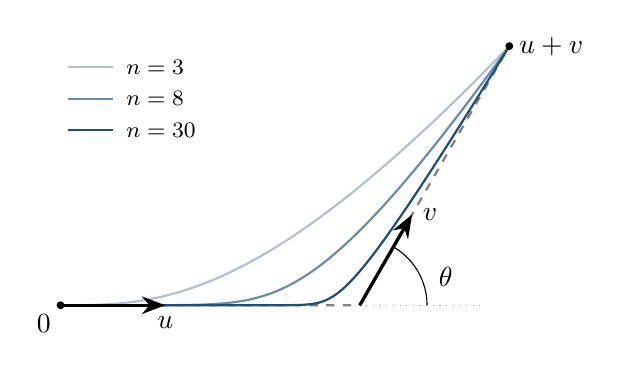
\begin{tikzpicture}[scale=0.95]
  % u = (1,0), v at 60 degrees, legs of length 4
  \coordinate (O) at (0,0);
  \coordinate (U) at (4,0);
  \coordinate (W) at ({4+4*cos(60)},{4*sin(60)});
  \draw[gray, dashed, thick] (O) -- (U) -- (W);
  \draw[gray!70, dotted] (U) -- (5.6,0);
  \draw[c1!35, thick] plot[domain=0:1, samples=120] ({4*\x+4*\x^3*cos(60)},{4*\x^3*sin(60)});
  \draw[c1!65, thick] (O) -- plot[domain=0.05:1, samples=150] ({4*\x+4*\x^8*cos(60)},{4*\x^8*sin(60)});
  \draw[c1, thick] (O) -- (2.4,0) -- plot[domain=0.6:1, samples=200] ({4*\x+4*\x^30*cos(60)},{4*\x^30*sin(60)});
  \draw[-{Stealth}, very thick] (O) -- (1.4,0) node[below] {$u$};
  \draw[-{Stealth}, very thick] (U) -- ($(U)+({1.4*cos(60)},{1.4*sin(60)})$) node[right] {$v$};
  \draw (4.9,0) arc (0:60:0.9);
  \node at (5.15,0.38) {$\theta$};
  \fill (O) circle (1.5pt) node[below left] {$0$};
  \fill (W) circle (1.5pt) node[right] {$u+v$};
  % legend in the empty upper-left corner
  \foreach \col/\lab [count=\k] in {c1!35/3, c1!65/8, c1/30} {
    \draw[\col, thick] (0.1,{3.6-0.42*\k}) -- (0.7,{3.6-0.42*\k});
    \node[anchor=west, font=\footnotesize] at (0.75,{3.6-0.42*\k}) {$n=\lab$};
  }
\end{tikzpicture}
\subcaption{The curves $\gamma_n$ for $\theta=\pi/3$.}
\end{subfigure}\hfill
\begin{subfigure}{0.48\textwidth}
\begin{tikzpicture}
\begin{axis}[paper, trig format plots=rad, xmin=0, xmax=3.2, ymin=0, ymax=2.1,
  xlabel={$\theta$}, legend pos=north west,
  xtick={0,0.7854,1.5708,2.3562,3.1416}, xticklabels={$0$,$\frac\pi4$,$\frac\pi2$,$\frac{3\pi}4$,$\pi$}]
  \addplot[c2, dashed, domain=0:3.1416, samples=120] {2*(sin(x/2))^2};
  \addplot[c1, domain=0:3.13, samples=200] {2*(sin(x/2))^2 + 4*(cos(x/2))^2*ln(cos(x/2))};
  \addplot[only marks, mark=o, mark size=2pt, black] coordinates {(0.5236,0.0045781) (0.7854,0.022549) (1.0472,0.068428) (1.5708,0.30675) (2.0944,0.80670) (2.3562,1.14425) (2.6180,1.50366)};
  \legend{$2\sin^2(\theta/2)$, $C(\theta)$, numerical ($n=10^6$)}
\end{axis}
\end{tikzpicture}
\subcaption{The two constants of Theorem~\ref{thm:angle}.}
\end{subfigure}
\caption[Corners of arbitrary angle]{Corners of arbitrary angle. (a)~As $n$ grows, $\gamma_n$
collapses onto the path $0\to u\to u+v$ (dashed), which turns by the angle $\theta$.
(b)~The coefficient $2\sin^2(\theta/2)$ of $\ln n/(n-1)$ and the constant $C(\theta)$. The
circles show $(n-1)\bigl(2-L_\theta(n)\bigr)-2\sin^2(\theta/2)\ln n$ at $n=10^6$.}
\label{fig:angle}
\end{figure}

\begin{table}[!htbp]
\centering
\caption[Numerical check of Theorem~\ref{thm:angle}]{Numerical check of
Theorem~\ref{thm:angle}. The last column is computed from $L_\theta(n)$ by direct quadrature
at $n=10^6$. It should equal $C(\theta)$ up to $O(\ln^2 n/n)\approx2\times10^{-4}$.}
\label{tab:angle}
\small
\begin{tabular}{cccc}
\toprule
$\theta$ & $2\sin^2(\theta/2)$ & $C(\theta)$ & $(n-1)\bigl(2-L_\theta(n)\bigr)-2\sin^2\frac\theta2\ln n$\\
\midrule
$\pi/6$  & 0.133975 & 0.0045910 & 0.0045781\\
$\pi/4$  & 0.292893 & 0.0225777 & 0.0225492\\
$\pi/3$  & 0.500000 & 0.0684769 & 0.0684278\\
$\pi/2$  & 1.000000 & 0.3068528 & 0.3067523\\
$2\pi/3$ & 1.500000 & 0.8068528 & 0.8066971\\
$3\pi/4$ & 1.707107 & 1.1444313 & 1.1442509\\
$5\pi/6$ & 1.866025 & 1.5038583 & 1.5036576\\
\bottomrule
\end{tabular}
\end{table}

%======================================================================
\section{A corner without a logarithm: the squircle}\label{sec:squircle}
%======================================================================

Let $Q(p)$ be the length of the arc $x^p+y^p=1$, $x,y\ge0$, and let
$P(p)=4Q(p)$ be the full perimeter. At $p=2$, $P=2\pi$.

\begin{theorem}\label{thm:squircle}
Let $K:=2\sqrt2\,\ln(1+\sqrt2)-2\ln 2=1.1066065994\ldots$. For every $p\ge2$,
\[
  \Bigl|\,Q(p)-\Bigl(2-\frac{K}{p}\Bigr)\Bigr|\le\frac{3}{p^2},
  \qquad\text{hence}\qquad
  \Bigl|\,P(p)-\Bigl(8-\frac{4K}{p}\Bigr)\Bigr|\le\frac{12}{p^2}.
\]
\end{theorem}

\begin{proof}
Parametrize the arc by $t\in(0,1)$ via $x=t^{1/p}$, $y=(1-t)^{1/p}$. Put $\eps=1/p\le\frac12$,
$a=t^{\eps-1}$ and $b=(1-t)^{\eps-1}$. Then $|x'|=a/p$ and $|y'|=b/p$, and by~\eqref{eq:taxicab}
(taxicab length $2$),
\[
  2-Q(p)=\frac1p F(\eps),\qquad F(\eps):=\int_0^1\Phi_\eps(t)\dd t,\qquad \Phi_\eps=a+b-\sqrt{a^2+b^2}.
\]

\emph{Step 1: $F(0)=K$.} At $\eps=0$, $a=1/t$ and $b=1/(1-t)$. Put $q=\sqrt{t^2+(1-t)^2}$. Then
$\Phi_0=(1-q)/(t(1-t))$, and $1-q=(1-q^2)/(1+q)=2t(1-t)/(1+q)$. So the integrand simplifies to
$\Phi_0(t)=2/(1+q)$. Substitute $w=2t-1$, so that $q^2=(1+w^2)/2$, and then $w=\sinh\phi$. With
$A=\operatorname{arsinh}1=\ln(1+\sqrt2)$,
\[
  F(0)=2\int_0^1\frac{\dd w}{1+\sqrt{(1+w^2)/2}}
  =2\sqrt2\int_0^{A}\frac{\cosh\phi}{\sqrt2+\cosh\phi}\dd\phi
  =2\sqrt2\,A-4\int_0^A\frac{\dd\phi}{\sqrt2+\cosh\phi}.
\]
With $\tau=\tanh(\phi/2)$, the last integral becomes
$\int_0^{\sqrt2-1}\frac{2\dd\tau}{(\sqrt2+1)-(\sqrt2-1)\tau^2}
=\ln\frac{\alpha+\tau}{\alpha-\tau}\Big|_{\tau=\sqrt2-1}=\frac12\ln2$, where
$\alpha=\sqrt2+1$. (Here we used $\tanh(A/2)=\sinh A/(1+\cosh A)=\sqrt2-1$.)
Hence $F(0)=K$.

\emph{Step 2: $|F(\eps)-K|\le3\eps$.} Since $\Phi_\eps(t)=\Phi_\eps(1-t)$, it suffices to consider
$0<t\le\frac12$. Write $r=\sqrt{a^2+b^2}$. Then $\partial\Phi/\partial a=1-a/r\in[0,1)$ and
likewise for $b$. Also $\partial_\eps a=a\ln t$ and $\partial_\eps b=b\ln(1-t)$. For
$t\le\frac12$ and $\eps\le\frac12$ we have $1\le b\le2$ and $a\ge t^{-1/2}$. Moreover
$(1-a/r)\,a=\frac{ab^2}{r(r+a)}\le\frac{b^2}{2a}$. Hence
\[
  |\partial_\eps\Phi_\eps(t)|\le\frac{b^2}{2a}|\ln t|+b|\ln(1-t)|\le2\sqrt t\,|\ln t|+2\ln2\le\frac4e+2\ln2<3.
\]
By the mean value theorem, $|\Phi_\eps(t)-\Phi_0(t)|\le3\eps$ for every $t$. Integrating over
$[0,1]$ gives $|F(\eps)-K|\le3\eps$. The result follows from
$Q(p)=2-F(1/p)/p$.
\end{proof}

Numerical evaluation of $F'(0)=\int_0^1\partial_\eps\Phi_\eps(t)|_{\eps=0}\dd t$ gives
$F'(0)=-0.5052381924\ldots$. This indicates that
$P(p)=8-4K/p+\kappa/p^2+o(p^{-2})$ with $\kappa=-4F'(0)=2.0209527696\ldots$, well within the
bound in Theorem~\ref{thm:squircle}; see Table~\ref{tab:sq} and Figure~\ref{fig:squircle}(b).

Figure~\ref{fig:squircle}(a) shows where $K$ comes from. Near the corner $(1,1)$, put
$x=1-\alpha/p$ and $y=1-\beta/p$. To leading order the equation $x^p+y^p=1$ becomes
$e^{-\alpha}+e^{-\beta}=1$, a single fixed curve that does not depend on $p$ (see
Section~\ref{sec:why}).

\begin{figure}[!htbp]
\centering
\begin{subfigure}{0.48\textwidth}
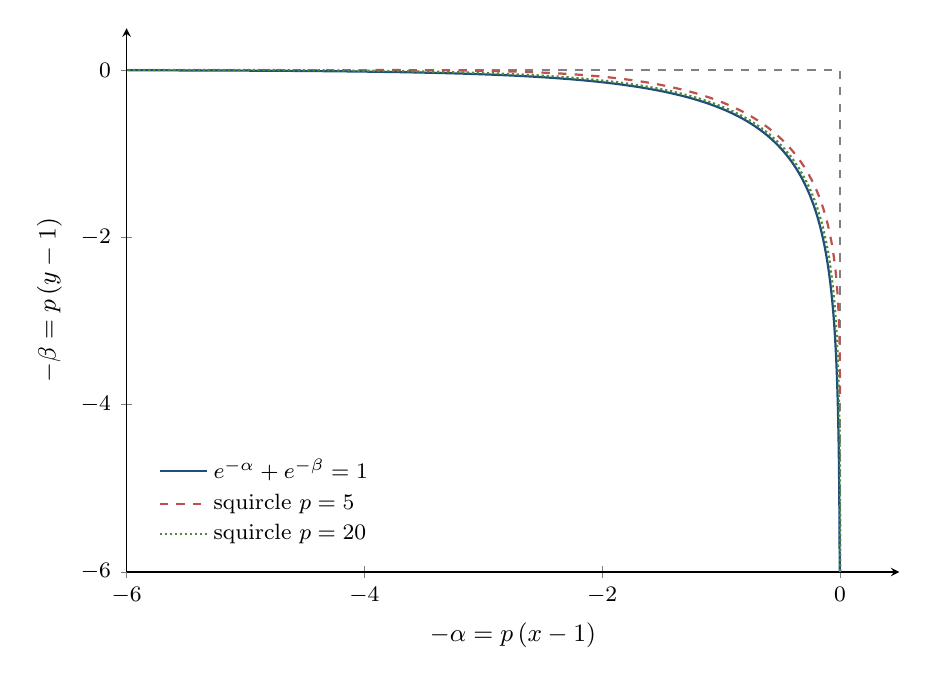
\begin{tikzpicture}
\begin{axis}[paper, xmin=-6, xmax=0.5, ymin=-6, ymax=0.5,
  xlabel={$-\alpha=p\,(x-1)$}, ylabel={$-\beta=p\,(y-1)$}, legend pos=south west,
  xtick={-6,-4,-2,0}, ytick={-6,-4,-2,0}]
  \draw[gray, dashed] (axis cs:-6,0) -- (axis cs:0,0) -- (axis cs:0,-6);
  \addplot[c1, domain=0.0025:0.9975, samples=400, variable=t] ({ln(t)}, {ln(1-t)});
  \addplot[c2, dashed, domain=0.0005:0.9995, samples=400, variable=t] ({5*(t^(1/5)-1)}, {5*((1-t)^(1/5)-1)});
  \addplot[c3, densely dotted, domain=0.0005:0.9995, samples=400, variable=t] ({20*(t^(1/20)-1)}, {20*((1-t)^(1/20)-1)});
  \legend{$e^{-\alpha}+e^{-\beta}=1$, squircle $p=5$, squircle $p=20$}
\end{axis}
\end{tikzpicture}
\subcaption{The corner, magnified by the factor $p$.}
\end{subfigure}\hfill
\begin{subfigure}{0.48\textwidth}
\begin{tikzpicture}
\begin{axis}[paper, xmin=0, xmax=0.52, ymin=3.3, ymax=4.6,
  xlabel={$1/p$}, ylabel={$p\,\bigl(8-P(p)\bigr)$}, legend pos=south west]
  \addplot[c1, domain=0:0.5, samples=2] {4.426426398 - 2.02095277*x};
  \addplot[only marks, mark=*, mark size=1.5pt, black] coordinates {(0.5,3.43363) (0.4,3.63324) (0.33333,3.76502) (0.25,3.92921) (0.2,4.02778) (0.16667,4.09364) (0.125,4.17621) (0.1,4.22592) (0.076923,4.27193) (0.0625,4.30076) (0.05,4.3258) (0.033333,4.35925) (0.02,4.38608) (0.01,4.40623) (0.001,4.42441)};
  \addplot[c2, dashed, domain=0:0.5, samples=2] {4.426426398};
  \legend{$4K-\kappa/p$, exact, $4K\approx4.4264$}
\end{axis}
\end{tikzpicture}
\subcaption{Rescaled perimeter defect.}
\end{subfigure}
\caption[The squircle near its corner, and its perimeter defect]{The squircle.
(a)~Near the corner $(1,1)$, magnified by the factor $p$, the squircle approaches the fixed curve
$e^{-\alpha}+e^{-\beta}=1$, which meets its asymptotes (the sides of the square) exponentially
fast. (b)~$p\,(8-P(p))$ tends to $4K$ as $p\to\infty$, with slope close to $-\kappa$
(Theorem~\ref{thm:squircle}).}
\label{fig:squircle}
\end{figure}

\begin{table}[!htbp]
\centering
\caption[Numerical values of the squircle perimeter]{Perimeter of the squircle
$|x|^p+|y|^p=1$ compared with Theorem~\ref{thm:squircle}.
The last column approaches $\kappa\approx2.02095$.}\label{tab:sq}
\begin{tabular}{rccc}
\toprule
$p$ & $P(p)$ & $8-4K/p$ & $p^2\bigl(P(p)-8+4K/p\bigr)$\\
\midrule
2    & 6.283185307180 ($=2\pi$) & 5.786786801 & 1.986\\
4    & 7.017697943564 & 6.893393401 & 1.989\\
10   & 7.577408317258 & 7.557357360 & 2.005\\
20   & 7.783710054121 & 7.778678680 & 2.013\\
50   & 7.912278464092 & 7.911471472 & 2.017\\
100  & 7.955937655831 & 7.955735736 & 2.019\\
1000 & 7.995575594378 & 7.995573574 & 2.021\\
\bottomrule
\end{tabular}
\end{table}

%======================================================================
\section{Why the logarithm?}\label{sec:why}
%======================================================================

Formula~\eqref{eq:taxicab} says that length is lost only while the curve
moves in a direction strictly between horizontal and vertical. A steep piece of the curve with slope
$s\gg1$ loses the fraction $g(s)\approx1$ of its horizontal extent. So the defect is
approximately the \emph{horizontal distance traveled while the curve is steep}.

For $y=x^n$, the slope exceeds $1$ exactly when $x\ge n^{-1/(n-1)}$. This is an interval of
length
\[
  1-n^{-1/(n-1)}=\frac{\ln n}{n}+O\!\left(\frac{\ln^2n}{n^2}\right).
\]
Near $x=1$ we have $x^n\approx e^{-n(1-x)}$. To climb from height $1/n$ (where the slope is about
$1$) to height $1$, the curve must advance horizontally by about $\ln(n)/n$. The
logarithm measures how many ``$e$-folds'' of height the curve climbs while steep. Equivalently,
$x^n$ approaches the vertical leg $x=1$ only logarithmically: at height $y$, its distance to
the leg is $\ln(1/y)/n$. Figure~\ref{fig:steep} shows this for $n=20$.

\begin{figure}[!htbp]
\centering
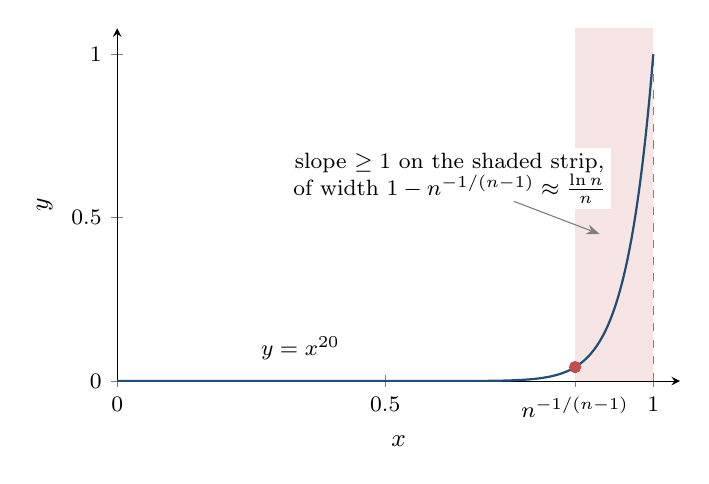
\begin{tikzpicture}
\begin{axis}[paper, width=0.72\textwidth, height=0.5\textwidth, xmin=0, xmax=1.05, ymin=0, ymax=1.08,
  xlabel={$x$}, ylabel={$y$}, xtick={0,0.5,0.8541,1}, xticklabels={$0$,$0.5$,$n^{-1/(n-1)}$,$1$},
  ytick={0,0.5,1}]
  \fill[c2!15] (axis cs:0.8541,0) rectangle (axis cs:1,1.08);
  \draw[gray, dashed] (axis cs:1,0) -- (axis cs:1,1);
  \addplot[c1, domain=0:1, samples=400] {x^20};
  \addplot[only marks, mark=*, mark size=1.8pt, c2] coordinates {(0.8541,0.04271)};
  \node[font=\footnotesize, align=center, fill=white, inner sep=2pt] at (axis cs:0.62,0.62)
    {slope $\ge1$ on the shaded strip,\\ of width $1-n^{-1/(n-1)}\approx\frac{\ln n}{n}$};
  \draw[-{Stealth}, gray] (axis cs:0.74,0.55) -- (axis cs:0.9,0.45);
  \node[font=\footnotesize, anchor=west] at (axis cs:0.25,0.1) {$y=x^{20}$};
\end{axis}
\end{tikzpicture}
\caption[Where the length defect of $x^n$ comes from]{Where the defect of $x^n$ comes from
($n=20$). The curve has slope at least $1$ only on the shaded strip. There it climbs from
height about $1/n$ (dot) to $1$, while moving horizontally by about $\ln n/n$. Almost all of
that horizontal movement is lost relative to the corner path.}
\label{fig:steep}
\end{figure}

The squircle behaves differently. Its steep part is confined to a neighborhood of size
$O(1/p)$ around the corner $(1,1)$. Put $x=1-\alpha/p$ and $y=1-\beta/p$. The equation
$x^p+y^p=1$ becomes, to leading order, $e^{-\alpha}+e^{-\beta}=1$: a single fixed curve,
blown down by the factor $1/p$. This curve approaches its two asymptotes \emph{exponentially}
fast, so its total ``diagonal travel'' is finite. The constant $K$ in
Theorem~\ref{thm:squircle} is exactly the taxicab defect of the curve
$e^{-\alpha}+e^{-\beta}=1$. (Parametrizing by $e^{-\alpha}=t$ reproduces the integral for
$F(0)$.)

In short, the defect is of order $1/n$ times the logarithm of the range of heights the curve
covers while steep. For the squircle this range is bounded. For $x^n$ it is a factor of
$n$.

%======================================================================
\section{Concluding remarks and open questions}\label{sec:conclusion}
%======================================================================

\subsection{Summary}
When a family of curves collapses onto a corner, the length defect measures how much
diagonal travel the curves do on the way. For the graph of $x^n$ the defect is
$(\ln n+1-\ln2)/(n-1)$ to first order. We derived this, and the complete asymptotic expansion,
from an exact Gamma-function formula (Theorem~\ref{thm:exact}). The logarithm persists for every
turning angle, with coefficient $2\sin^2(\theta/2)$ (Theorem~\ref{thm:angle}). It is absent for
the squircle, whose perimeter defect is $4K/p$ (Theorem~\ref{thm:squircle}). The difference comes
down to how fast each curve approaches the sides of the corner: logarithmically for $x^n$,
exponentially for the squircle.

\subsection{Open questions}

\begin{question}
Is there a closed form for the second squircle constant
$\kappa=\lim_{p\to\infty}p^2\bigl(P(p)-8+4K/p\bigr)=2.02095276965\ldots$? It equals
$-4F'(0)$, where $F'(0)=\int_0^1\partial_\eps\Phi_\eps|_{\eps=0}\dd t$. This is an integral of
logarithms against algebraic functions, so we expect dilogarithms. An integer-relation search
against $\pi^2$, $\ln^2 2$, $\ln^2(1+\sqrt2)$, $\sqrt2\ln2\ln(1+\sqrt2)$, $\ln2$, and
$\sqrt2\ln(1+\sqrt2)$ found no relation.
\end{question}

\begin{question}
Theorem~\ref{thm:exact} rests on the Mellin transform of $g=h_0$. Find the analogous exact
formula for general angles, based on the Mellin transform of $h_c$ in~\eqref{eq:hc}. We expect
Legendre functions of $\cos\theta$.
\end{question}

\begin{question}
The heuristic of Section~\ref{sec:why} suggests the following. Let $f:[0,1]\to[0,1]$ be smooth
and increasing, with $f(0)=0$, $f(1)=1$ and $f'(1)>0$. Then the graph of $f^n$ should satisfy
$2-\operatorname{length}(f^n)\sim\ln n/\bigl(f'(1)\,n\bigr)$. Prove this, and find the next
term.
\end{question}

\begin{question}
What happens in higher dimensions? For example, how does the area of the graph of
$z=x^ny^n$ over $[0,1]^2$ approach its limit?
\end{question}

\subsection{Code availability}
All numerical values in this paper were computed with 30--50 significant digits using
\texttt{mpmath}. The accompanying script \texttt{verify.py} recomputes them. It checks
Theorem~\ref{thm:exact} against direct quadrature, the expansions of
Corollary~\ref{cor:asymp}, the constants $C(\theta)$ and $K$, and
Tables~\ref{tab:xn}--\ref{tab:sq}. The script and the \LaTeX{} source of this paper are available
under the MIT license at \url{https://github.com/zishaan1911/arc-length-of-xn}.

\begin{thebibliography}{9}

\bibitem{BBI}
D.~Burago, Y.~Burago, and S.~Ivanov,
\emph{A Course in Metric Geometry},
Graduate Studies in Mathematics~33, American Mathematical Society, 2001.

\bibitem{DLMF}
F.~W.~J.~Olver et al., eds.,
\emph{NIST Digital Library of Mathematical Functions},
\url{https://dlmf.nist.gov/} (Chapters~5 and~15).

\bibitem{FGD}
P.~Flajolet, X.~Gourdon, and P.~Dumas,
Mellin transforms and asymptotics: harmonic sums,
\emph{Theoretical Computer Science} \textbf{144} (1995), 3--58.

\bibitem{Gardner}
M.~Gardner,
Piet Hein's superellipse,
in \emph{Mathematical Carnival}, Vintage, New York, 1977.

\bibitem{MSE}
Math StackExchange, question 4187181,
``Arc length of $x^n$ found using hypergeometric function and series,''
\url{https://math.stackexchange.com/questions/4187181}.

\bibitem{MRL}
Y.~Montilla, R.~O.~Rodriguez, and B.~Linares,
On the arc length of a supercircle and a hypergeometric formulation of~$\pi$,
preprint, arXiv:2607.04592, 2026.

\bibitem{RM}
R.~O.~Rodriguez and Y.~Montilla,
Hypergeometric series representations for the perimeter of Lam\'e superellipses,
preprint, arXiv:2607.09048, 2026.

\end{thebibliography}

\end{document}
